% A Dedekind cut of the rationals at the gap where a square root of 2 would sit.
\begin{tikzpicture}[x=0.92cm,y=1cm]
  \draw[line width=1.15pt,MidnightBlue] (0.2,0)--(4.85,0);
  \draw[line width=1.15pt,BurntOrange] (5.55,0)--(10.3,0);
  \draw[dashed,thin,MidnightBlue] (5.2,-0.72)--(5.2,1.28);
  \node[above,font=\small] at (5.2,1.28) {$\sqrt{2}\notin\Q$};
  \fill[MidnightBlue] (0.7,0) circle (1.7pt);
  \fill[MidnightBlue] (2.15,0) circle (1.7pt);
  \fill[MidnightBlue] (3.45,0) circle (1.7pt);
  \fill[MidnightBlue] (4.45,0) circle (1.7pt);
  \node[below=3pt,font=\scriptsize] at (0.7,0) {$1$};
  \node[below=3pt,font=\scriptsize] at (2.15,0) {$\tfrac75$};
  \node[below=3pt,font=\scriptsize] at (3.45,0) {$1.4$};
  \node[below=3pt,font=\scriptsize] at (4.45,0) {$1.41$};
  \fill[BurntOrange] (5.95,0) circle (1.7pt);
  \fill[BurntOrange] (7.15,0) circle (1.7pt);
  \fill[BurntOrange] (8.45,0) circle (1.7pt);
  \fill[BurntOrange] (9.7,0) circle (1.7pt);
  \node[below=3pt,font=\scriptsize] at (5.95,0) {$1.42$};
  \node[below=3pt,font=\scriptsize] at (7.15,0) {$\tfrac32$};
  \node[below=3pt,font=\scriptsize] at (8.45,0) {$2$};
  \node[below=3pt,font=\scriptsize] at (9.7,0) {$3$};
  \node[font=\scriptsize,anchor=south] at (2.4,0.42) {square below $2$};
  \node[font=\scriptsize,anchor=south] at (7.9,0.42) {square above $2$};
\end{tikzpicture}
